\documentclass[]{article}

\usepackage[pdftex]{graphicx}
\usepackage{listings}
\usepackage[top=1in, bottom=1in, right=1.25in, left=1.25in]{geometry}
\usepackage{hyperref}

\begin{document}

	% Title Page
	\begin{titlepage}



		\title{\textbf{Bucknell ProPANE Final Report}}
		\author{BU ProPane Team:\\Griffin Dunn\\Colin Madigan\\Phillip Stahlfeld\\\\Clients:\\Dr. Robert Gabauer\\Dr. Robert Midkiff\\\\Advisor:\\Dr. Matthew Watkins}
		\date{April 29, 2013}
		\maketitle



		
		
		\thispagestyle{empty}
		\noindent
		The goal of this report is to document the major technical aspects of the ProPANE system and the process used to make the major technical decisions. 
		
		
		
	\end{titlepage}
	
	\thispagestyle{empty}
	
	
	% Begin  Real  Document
	\tableofcontents
	\newpage
	
	
	\setcounter{page}{1}
	\thispagestyle{empty}
	
	\section{Project Overview}
		One of the problems that professors at Bucknell University face is that they do not have a record of what was actually presented on whiteboards during their lectures. Despite having every lecture planned out on paper, there is still the problem of when a student asks a question that requires further explanation. The material displayed on the board that is not on a professor's written plan becomes lost once the board is erased. As seen in Figure \ref{fig:cive-notes}, some professors have found ways to keep track of some of this information, but these methods can consume unnecessary portions of class. Professors are not the only ones who require a means for capturing the information displayed on boards. Some students are not capable of taking notes themselves and Bucknell is legally required to provide a means for them to obtain copies of the information presented on boards in class. Currently, the solution to this problem is to assign a note-taker who is responsible for recording information presented on the board and then sending a copy of the notes to the professor so that the notes can be distributed to students who are incapable of taking notes themselves. This places extra stress on the note-taker because the notes have to be copied exactly as from the board (including all of the information, in the proper layout, without shorthand notation, and following the same color scheme). Essentially, both students and professors need a way of capturing all of the information written on whiteboards during lectures. The goal of the Bucknell University Professional Portable Automatic Note Extraction (BU ProPANE) system is to solve this problem by automatically capturing digital images of the information presented on the board and sending the images to professors.\\
		\\
		This project is especially relevant to anyone concerned with learning disabilities because it simplifies the process for assisting students with certain disabilities. For example, according to Dr. Midkiff of Bucknell University, some students have a difficult time reading colored writing on a white background. By applying a red filter to digital images of a whiteboard, the colored writing will be set on a red background and allow the student to read the information. There are numerous other ways that digital image manipulation can make information accessible to students whose disabilities prohibit them from learning the information presented on a whiteboard during a class.\\
		\\
		One of the obvious solutions to this problem is to use SMART boards which are essentially large touch screens, but this would mean that SMART boards would have to be installed in every classroom where a student with learning disabilities has class. The goal of BU ProPANE is to create a portable system that can be used in any classroom with very little setup time. Ideally, this will reduce costs and interfere less with the way professors currently teach classes. 
		
		% Image of Professor Gabauer's lecture notes
		\begin{figure}[h]
      			\centering
      			\includegraphics[scale=0.2]{./images/cive-notes.png}
			\caption{Image of civil engineering lecture notes. Orange note is an example of how lecture notes are recorded and altered. Image courtesy of Doug Gabauer 2012.}
			\label{fig:cive-notes}
   		 \end{figure}

	\section{Background}
	\subsection{Signal Processing}

According to the IEEE Signal Processing Society, 
		{\quotation {\sl \noindent Signal processing is the enabling technology for the generation, transformation, and interpretation of information. It comprises the theory, algorithms, architecture, implementation, and applications related to processing information contained in many different formats broadly designated as signals. Signal refers to any abstract, symbolic, or physical manifestation of information with examples that include: audio, music, speech, language, text, image, graphics...  \\
\noindent Signal processing uses mathematical, statistical, computational, heuristic, and/or linguistic representations, formalisms, modeling techniques and algorithms for generating, transforming, transmitting, and learning from analog or digital signals, which may be performed in hardware or software. Signal generation includes sensing, acquisition, extraction, synthesis, rendering, reproduction and display. Signal transformations may involve filtering, recovery, enhancement, translation, detection, and decomposition. The transmission or transfer of information includes coding, compression, securing, detection, and authentication. Learning can involve analysis, estimation, recognition, inference, discovery and/or interpretation.}}  \cite{IEEESPS} \\

\noindent Signal processing applies to both analog and digital signals.  Analog signals are sets of continuous values, and can be directly processed using both linear and non-linear electronic circuits.  These signals can be sampled to obtain a signal with the same values, but only at discrete points over an interval in time.  These signals can also be directly processed with electronic circuitry, but they can also be digitized to create digital signals.  Digital signal processing can be done conveniently on computers, or on dedicated digital circuits such as application-specific integrated circuits (ASICs) and field-programmable gate arrays (FPGAs).  For this project, we are interested in digital signal processing, and specifically the field of image processing. \\

		\subsection{Image Processing}

Digital images are electronic representations of physical media, such as photographs, texts, artwork and more.  The digital image is sampled and mapped as a grid of pixels.  Each pixel is assigned a tonal value (black, white, shades of gray or color) which is represented in binary.  The bits representing each pixel are stored by a computer and can be compressed via mathematical reduction of some kind.  To view an image, the bits are interpreted and read by the computer to produce an analog version for display. \\ 

\begin{figure}[h]
      			\centering
      			\includegraphics[scale=0.75]{./images/research_image_processing_1}
			\caption{A bitonal image, where each pixel is assigned either a 0 or 1 to represent color.}
			\label{fig:research_image_processing_1}
   		 \end{figure}

\noindent Digital images can be displayed with different resolutions.  Resolution is the ability to display fine spatial detail.  In general, resolution increases with sampling frequency.  Common units of resolution are dots-per-inch (dpi) and pixels-per-inch (ppi).   \\ 

\noindent The number of bits used to define each pixel is defined as the bit depth.  The greater the bit depth, the greater the number of tones can be represented.  Normally, a color image is represented by a bit depth of 8 to 24.  In a 24-bit image, the bits are often divided into red, green and blue, with 8 bits for each color.  Other colors are obtained from combinations of those bits.  In a 24-bit image, there are 16.7 million color values ($2^{24}$).  	\\ 

\noindent To reduce image file size for storage, processing and transmission, compression is used.  Compression techniques use algorithms to abbreviate the binary code in an uncompressed image.  Both lossless and lossy forms of compression exist. Lossless schemes abbreviate the binary code without discarding any information so that the decompressed image is bit-for-bit identical to the original.  Lossy schemes average and discard the least significant information based on an understanding of visual perception.  JPEG is a common lossy compression scheme.  Some lossy-compressed images may appear identical to the raw image, and are considered ``visually lossless''.  \cite{cornell} 

\begin{figure}[h]
      			\centering
      			\includegraphics[scale=0.75]{./images/research_image_processing_2}
			\caption{Example of a ``visually lossless'' compressed image.  The full images look the same regardless of compression level, but the zoomed in images get blurrier as compression increases.}
			\label{fig:research_image_processing_2}
   		 \end{figure}

\subsection{Image Processing Tools}

\noindent Image processing can be implemented using a variety of different tools.  There are programs, such as Adobe Photoshop, which provide users with a graphical user interface and on-screen tools to use to edit their images.  While programs like this can achieve desirable high-quality results, the process can be time-consuming for an individual image, and must be repeated for each subsequent image.  A far better option for similar processing of a large quantity of images is to use a programming language with an image processing library.  The user can write a program which performs desired effects on any number of images.  A variety of libraries exist to add image processing features to many programming languages.  The libraries listed in this section are for common programming languages and seem to have some or all of the functionality required for the ProPANE project.  \\ 

\noindent {\sl Eutecus Signal and Image Processing Library} \cite{eutecus} \\

\noindent A collection of general-purpose, optimized C++ routines and classes, along with utility classes to aid image and video file manipulation.  These routines are usually used in computationally intensive real-time applications, where optimal execution speed is critical.  For use, licensing rights must be purchased. \\

\noindent {\sl OpenCV} \cite{opencv} \\

\noindent A free library of programming functions for real time computer vision, originally developed by Intel.  It has interfaces for C, C++, Python, and soon Java, running on Windows, Linux, Android and Mac.  There are over 2500 algorithms optimized for image processing.  \\

\noindent {\sl Aforge.NET Framework} \cite{aforge1} \\

\noindent A free, open-source C\# framework, containing libraries for image processing, robotics, and more.  The image processing library, AForge.Imaging, contains different image processing routines, aimed to help with image enhancement and processing.  \\

\noindent {\sl Python Imaging Library} \cite{pil} \\

\noindent A free library which adds image processing capabilities to the Python interpreter.  It supports many file formats and provides powerful image processing and graphics capabilities. \\

\noindent {\sl VIPS} \cite{vips} \\

\noindent A free image processing system.  Good with large images, with many CPUs.  It needs little memory and runs quickly compared to many libraries.  The library can be used from C, C++, command line, Python, Ruby, JavaScript and others.  Includes a GUI for Photoshop-style editing. Works on Linux/Unix, Windows 7 and MacOS. \\

\noindent {\sl MATLAB Image Processing Toolbox} \cite{matlab_ipt} \\ 

\noindent A comprehensive set of reference-standard algorithms and graphical tools.  For image processing, analysis, visualization, and algorithm development.  Features include image enhancement, deblurring, feature detection, noise reduction, segmentation, geometric transformations, and image registration.  Using the Image Acquisition Toolbox, images can be acquired directly from a camera and read into MATLAB or Simulink. \cite{matlab_iat} \\ 


\noindent {\sl Mathematica} \cite{mathematica} \\

\noindent Mathematica provides built-in support for programmatic modern industrial-strength image processing, fully integrated with its powerful mathematical and algorithmic capabilities.  Mathematica's symbolic architecture and notebook paradigm allow images in visual form to be included and manipulated directly both interactively and in programs.


	\subsection{Image Processing Techniques}

\noindent Many techniques currently exist for processing images in numerous different ways.  The techniques in this section seem relevant to the image processing necessary for the ProPANE system. \cite{ndt} \\ \\
{\sl Image Analysis- \\ \indent Extract information from the image} 
			\begin{itemize} 
				\item{\textbf{Image statistics:}} Calculates the maximum, minimum, average, standard deviation, variance, median, and mean-square intensities of the image data					
				\item{\textbf{Gray-scale mapping:}} Alters the mapping of the intensity of pixels in a file to match the intensity displayed on a computer screen 
				\item{\textbf{Image extraction:}} Extracts a portion or all of an image and creates a new image with the selected area 
				\item{\textbf{Slice:}} Plots intensity versus position for any direction. Lists intensity versus pixel location from any point along the slice
			\end{itemize} 
{\sl Convolution and Noise Filtering- \\ \indent Decrease noise by diminishing statistical deviations}
			\begin{itemize}
				\item{\textbf{High-pass filter:}} Emphasizes regions with rapid intensity changes
				\item{\textbf{Low-pass filter:}} Smooths images, blurs regions with rapid change
				\item{\textbf{Adaptive smoothing filter:}} Sets pixel intensity to a value between original and mean values, corrected by degree of noisiness. Good for decreasing statistical, especiall signal-dependent noise
				\item{\textbf{Median filter:}} Sets pixel intensity to the median intensity of pixels in a neighborhood. Excellent for eliminating intensity spikes
				\item{\textbf{Sigma filter:}} Sets pixel intensity equal to the mean of the intensities in a neighborhood within two of the mean.  Good for signal-independent noise
			\end{itemize}
{\sl Edge Detection- \\ \indent Sharpen intensity-transition regions}	
			\begin{itemize}
				\item{\textbf{First-difference:}} Subtracts intensities of adjacent pixels.  Emphasizes noise as well as desired changes. 
				\item{\textbf{Sobel operator:}} Weighs inner pixels twice as heavily as corner values.  Calculates intensity differences
			\end{itemize}
{\sl Enhancement- }
			\begin{itemize}
				\item{\textbf{Histogram equalization:}} Redistributes the intensities of the image
			\end{itemize}

\subsection{Learning Disabilaties}
        \subsubsection*{Introduction}
One of the major motivating factors behind designing our image capturing system is to help meet the needs of students with disabilities. The term "students with disabilities" is a very broad term, however, so we would like to use the following section to help describe some of the things that mildly disabled students have trouble with at Bucknell, and would therefore need our system to capture information presented on the board for them. \\
Disabilities that students might have that impair their ability to take notes: \cite{disability}
    \begin{itemize}
        \item Visual Impairments
        \begin{itemize}
            \item May be fully blind and need notes translated into Braille
            \item May not see well and need large print letters
            \item May have trouble copying information from whiteboards, projectors, etc.
            \item May have trouble seeing certain colors when framed by a white or black background
        \end{itemize}
        \item Specific Learning Disabilities
        \begin{itemize}
            \item Reading disability
            \item Writing disability
            \item Spelling disability
            \item Inability to copy what they see
            \item Inability to write what they hear
            \item Inability to write legibly
            \item Number reversal problems
        \end{itemize}
        \item Mobility Impairments
        \begin{itemize}
            \item Physically unable to write
            \item Physically unable to write quickly
            \item May be unable to effectively handle a writing implement
        \end{itemize}
        \item Partial or full loss of hearing
    \end{itemize}

\noindent This is just a small portion of the many disabilities faced by students in universities around the world. We hope to help them by giving them full access to all information presented on boards during lectures. By providing easily accessible, easily modifiable images, we hope to help even the playing field for students with disabilities.
Secondary goals of our project will help to make the learning process even easier. Some students get distracted if they see more than one line of text at a time. If we have enough time we will help these students by providing slide bars that will cover portions of the images that students are not currently viewing. This and many other minor features are things that we will accomplish if we have free time after completing our primary objectives. 
		
		
	% Basically just copied tech spec into here	
	\section{Specification}
		The following subsections contain the specifications created in the fall for this project.
		\subsection{Overview}
			The goal of this project is to create a system that captures information written on whiteboards throughout the course of a class. The system should be useable by professors during a standard lecture. The system must be portable so that it can be transported from classroom to classroom.
			
		\subsection{System Breakdown}
			The ProPANE system will be composed of two subsystems: the capture system and the analysis system. There will be a single analysis system for multiple capture systems. This ensures a centralized location for data storage and accessibility.
			
			\subsubsection{Capture System}
				The responsibility of the capture system is to record all of the information presented on a whiteboard during a class and send it to the analysis system. The capture system will be composed of the capture device and any other components. The capture device is responsible for actually taking the pictures of the whiteboard.\\
				\\
				There are no requirements placed on the resolution of the images generated by the capture system because the research into this field showed that a camera from 10 years ago was capable of generating images at a high enough quality under similar conditions. 
				
			\subsubsection{Analysis System}
				The responsibility of the analysis system is to receive images from the capture system and identify/construct key frames. The analysis system will allow professors to browse all images from the capture system, browse key images, and export selected images. 
				
		\subsection{Use Case}
			The following steps show an end-to-end high level description of how the ProPANE system will be used.
			\begin{enumerate}
				\item Setup capture system in classroom
				\item Start the capture system
				\item Use whiteboard during class
				\item Stop the capture system 
				\item Browse images on analysis system
				\item Select desired images
				\item Export images to desired location
			\end{enumerate}			
			The analysis system will be designed to ease browsing of images described in step 5 by identifying key frames. The idea behind these frames is that they show the maximum amount of information that is on the board before it is erased and used again. 
			
	
		\subsection{List of Deliverables}
		
			Software source code\\
			Users guide\\
			Fully assembled capture system\\
			Fully assembled/installed analysis system\\
		
		\subsection{Setup}
				
			\subsubsection{Maximum Time Required}
				\textbf{Priority Level: MEDIUM}\\
				The maximum time required to prepare the capture system for recording shall not exceed 5 minutes. This requirement exists to ensure that setting up the system does not interfere with class time.\\
				\emph{This requirement will be verified through a demonstration of a third party setting up the system in fewer than 5 minutes.}
		
		\subsection{Capabilities}
			
			\subsubsection{Information Capture}
				\textbf{Priority Level: HIGH}\\
				The ProPANE system shall capture all of the information written on a board and within the capture field provided that there exists a clear line of sight from the capture device to the information for a minimum of 5 continuous seconds. This requirement exists to ensure that no information is lost.\\
				\emph{This requirement will be verified through a test of covering a portion of a board for all but 5 seconds and ensuring that the system captured all of the board. }
	
	
		\subsection{Operating Specifications}
			
			\subsubsection{Minimum Distance from Board}
				\textbf{Priority Level: HIGH}\\
				The minimum operating distance from board for the capture system shall not exceed 220 inches. This requirement exists to insure that the capture system can be used in the majority of rooms in the Dana Engineering and Breakiron buildings on the campus of Bucknell University.\\
				\emph{This requirement will be verified through an examination of the "Operating Parameters" section of the user manual and determining that the minimum operating distance is no greater than 220 inches.}
				
			
			\subsubsection{Maximum Distance from Board}
				\textbf{Priority Level: HIGH}\\
				The maximum operating distance from board for the capture system shall not be less than 60 inches. This requirement exists to insure that the capture system can be used in the majority of rooms in the Dana Engineering and Breakiron buildings on the campus of Bucknell University.\\
				\emph{This requirement will be verified through an examination of the "Operating Parameters" section of the user manual and determining that the minimum operating distance is no less than 60 inches.}
		
		\subsection{Dimensions}
			
			\subsubsection{Maximum Weight}
				\textbf{Priority Level: MEDIUM}\\
				The total weight of the capture device shall not exceed 2.5 kg. This requirement exists to maintain the goal of portability. Professors must be able to carry the device to classes and weight should not be an issue. \\
				\emph{This requiment will be tested by weighing the system and verifying that its weight is less than 2.5 kg.}
				
			
			\subsubsection{Maximum Size}
				\textbf{Priority Level: MEDIUM}\\
				The capture device shall fit inside of a cube with 0.75 m sides in its most collapsed and fully assembled state. This requirement exists to maintain the goal of portability. Professors must be able to carry the device through door frames. \\
				\emph{This requirement will be tested by ensuring that the final product can fit inside of a box with 0.75 m sides.}

		\subsection{Operating System}
			
			\subsubsection{Analysis System}
				\textbf{Priority Level: LOW}\\
				The analysis system shall support the Ubuntu 10.04 operating system. This requirement exists to ensure that the software can be run on a free-of-cost operating system. \\
				\emph{This requirement will be verified by developing the analysis system on the Ubuntu 10.04 operating system.}
				
		
		\subsection{File Formats}
			
			\subsubsection{Proprietary Formats}
				\textbf{Priority Level: LOW}\\
				The ProPANE system shall generate images that are in an open format (no proprietary formats). This requirement exists to ensure that the images can be viewed with free-of-cost software. \\
				\emph{This requirement will be verified by demonstrating that the output file formats are in an open format.}
				
			
			\subsubsection{Editable}
				\textbf{Priority Level: HIGH}\\
				The images generated by the ProPANE system shall be editable---to the extent of rotating and cropping---through the use of a free-from-cost editor. This requirement exists to ensure that professors have the ability to share selected portions of the captured images with their classes.\\
				\emph{This requirement will be verified through a demonstration of image rotation and cropping utilizing a free image editor.}
				
				
		\subsection{Capture System}
			
			\subsubsection{Starting Mechanism}
				\textbf{Priority Level: LOW}\\
				The mechanism for starting the capture system shall be simple enough to use as to require no special training aside from reading the user manual. This requirement exists to ensure that any professor will have the ability to use the system.\\
				\emph{This requirement will be verified by having a third party with no special training start the capture system with only the help of the user manual}
				
			
			\subsubsection{Stopping Mechanism}
				\textbf{Priority Level: LOW}\\
				The mechanism for stopping the capture system shall be simple enough to use as to require no special training aside from reading the user manual. This requirement exists to ensure that any professor will have the ability to use the system.\\
				\emph{This requirement will be verified by having a third party with no special training start the capture system with only the help of the user manual}
				
				
		\subsection{Analysis System}
			
			\subsubsection{Image Browsing}
				\textbf{Priority Level: HIGH}\\
				The analysis system shall provide a mechanism for accessing the identified key images. This requirement exists to ensure that the end user does not have to browse all of the images taken to find the key images by hand.\\
				\emph{This requirement will be verified through a demonstration of the system showing that key images were identified and referenced in some fashion.}
				
			\subsubsection{Export System}
				\textbf{Priority Level: HIGH}\\
				The analysis system shall provide a graphical interface for exporting image files to a specified location. This requirement exists to ensure that the images can be shared without difficulty.\\
				\emph{This requirement will be verified through a demonstration of the system showing that images can be exported to a specified folder.}
				
		\subsection{Additional Features}
				This section contains a collection of features that are not required for the ProPANE project, but have been formally requested by the clients for the next iteration of the project.
			
			\subsubsection{Multiple Boards}
				The ProPANE system shall be able to capture information from more than one board in a classroom.
			
			\subsubsection{Blackboards}
				The ProPANE system shall be effective for capturing information on blackboards as well as whiteboards. 
				
			\subsubsection{Browsing}
				The ProPANE system shall provide an interface for browsing collected images.
				
			\subsubsection{Editing}
				The ProPANE system interface shall provide features for image editing.
				

	\section{Specification Verification}
	
	
	
		\subsection{Results from Specification Testing}
			The table in Figure \ref{fig:specreview} shows the results from the testing done to verify that the deliverable met the proposed specifications. 
			
			% Review of technical specifications 
			\begin{figure}
				\centering
				\includegraphics[scale=0.78]{images/technicalspecificationreview.pdf}	
				\caption{Table showing that all technical specifications for this project have been met. Additionally, there is an extra feature (color normalization) that was implemented and tested for the system.}	
				\label{fig:specreview}
			\end{figure}
			
		\subsection{Adjustments to Specifications}
			Specification 5.1.1 was altered from supporting Ubuntu 10.04 to supporting Ubuntu 12.04. This adjustment was made to allow for easier installation of required software for the analysis system. These pieces of software are listed below:
			\begin{itemize}
				\item NumPy
				\item SciPy
				\item Samba Server
			\end{itemize}
			
		\subsection{Additional Specifications Looking Back}
			If we did this project again, we would add the following specifications for how the system should function:
			\begin{itemize}
				\item A key image shall be generated when at least 5\% of all writing on the board and within the capture field has changed or been erased.
				\item The system shall be capable of capturing all information written on a board with dimensions 6 feet by 4 feet.
			\end{itemize}
			The first requirement would be used to ensure that the system is actually generating key images correctly. The second requirement would be used to ensure that the system is actually capturing a usable amount of board space.
					
	\section{Design Evolution}
		
		\subsection{System Architecture}
		
		
			The high level view of the system is depicted in Figure \ref{img:concept-of-operation}. The system in broken down into the following three subsystems:
			\begin{itemize}
				\item Capture System: responsible for capturing images of the whiteboard
				\item Analysis System: responsible for processing the images from the capture system
				\item Backend System: responsible for detecting new capture sets and file system manipulations
			\end{itemize}
			\noindent
			Each of these subsystems is discussed in greater detail in the following sections of the document. 
			
			\begin{figure}[h]
				\centering
				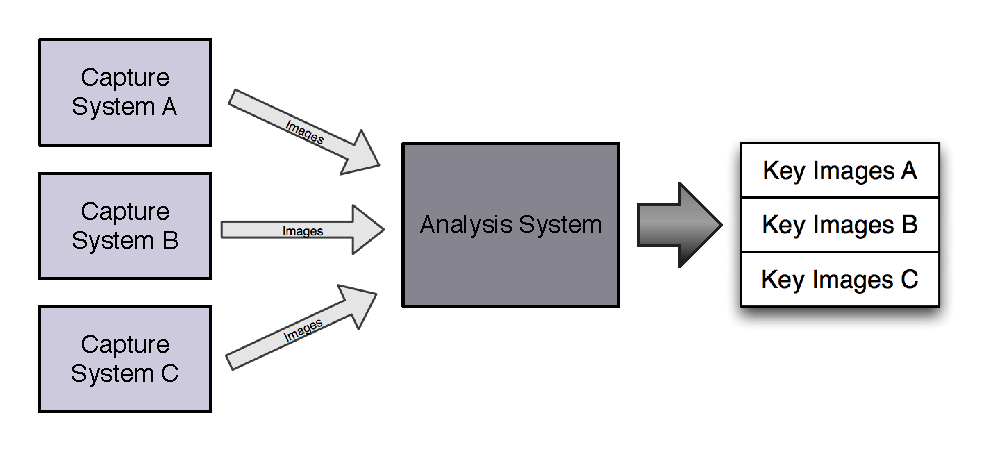
\includegraphics[scale=0.8]{images/concept-of-operation.eps}
				\caption{This figure shows the high level concept of operation where capture systems feed images into the analysis system, which then produces a set of key images. There is a one-to-one relationship between a capture set and a set of key images.}		
				\label{img:concept-of-operation}
			\end{figure}
			
		\subsection{Capture System}
		
			\subsubsection{Capture Device Decision process}
				The requirements from the technical specifications that the capture system had to meet are listed below:
				\begin{itemize}
					\item The maximum time required to prepare the capture system for recording shall not exceed 5 minutes.
					\item The ProPANE system shall capture all of the information written on a board and within the capture field provided that there exists a clear line of sight from the capture device to the information for a minimum of 5 continuous seconds.
					\item The total weight of the capture device shall not exceed 2.5 kg.
					\item The capture device shall fit inside of a cube with 0.75 m sides in its most collapsed and fully assembled state. 
				\end{itemize}
				
				\noindent
				The ProPANE team compared the following list of capture devices against the specifications in an attempt to determine the optimal one for the project:
				\begin{itemize}
					\item Logitech HD Pro Webcam C920
					\item Nikon CoolPix S800C
					\item Samsung Galaxy Camera
					\item Samsung WB150F Smart Wi-Fi Digital Camera
					\item Canon PowerShot G15 connected via USB to laptop
				\end{itemize}
				
				\noindent
				The Logitech webcam was ruled out due to lack of resolution (violating the requirement for capturing all of the information on the whiteboard). The Nikon CoolPix S800C was ruled out due to the fact that it had an automatic shutdown timer so that it would not be capable of capturing images throughout an entire lecture. The remaining three systems would all meet specification so the following criterion were used to select the optimal capture device:
				\begin{itemize}
					\item Decreasing the number of steps in the setup will increase usability
					\item Decreasing number of discrete components in system will increase usability
				\end{itemize}
				The Samsung WB150F (Galaxy Camera without Android and touchscreen) would require a battery pack and a laptop to control it via Wi-Fi. The Canon PowerShot G15 would require a laptop to control it. The Samsung Galaxy Camera (see Figure \ref{img:galaxy-camera} could operate entire independently so it was the logical choice for the capture device. 
				
				\begin{figure}[h]
					\centering
					\includegraphics[scale=0.45]{images/galaxy-camera.jpg}
					\caption{Three views of the Samsung Galaxy Camera. The left view shows the camera running a full Android 4.1 operating system. The other two images show that it has a telescopic lense that will allow for physical zooming so that the camera can be placed anywhere in the classroom and still capture high resolution images.}		
					\label{img:galaxy-camera}
				\end{figure}
			
			\subsubsection{Android App v1}
				The first iteration of the capture system app allowed the user to start capturing images and to stop the capture. The images were all timestamped and were taken every 5 seconds. They were stored in the Pictures directory all together and were not separated from any of the other capture sets.
				
			\subsubsection{Android App v2}
				The second iteration of the capture system app created a timestamped directory every time a new capture was started and placed the images from that capture into the directory. This separated the captures from each other. The problem with this version of the app is that when the screen turned off, it would stop the app. Adjusting the settings for the camera made it possible to keep the screen on at all times, but the battery drain would not allow for captures of longer classes.
				
			\subsubsection{Android App v3}
				The third iteration of the capture system utilized a wakelock to keep the app running even when the screen turned off. Zoom functionality was also added to the app so that the camera could be placed in different places is the room. This version was buggy and if the app was closed the wrong way, the camera became unreachable without a restart. 
				
			\subsubsection{Android App v4}
				The fourth iteration of the capture system used the onPause, onStop, and onResume calls in Android to correctly lock and release the camera so that if the app is closed at any time, the camera will still be useable without a restart. There was also a button added to this version to toggle between high resolution and low resolution capture modes. This feature was requested for the keystone correction feature of the analysis system. This was the final version of the app that was developed since it went beyond meeting specification and the team wanted to focus more on the analysis system improvements. The final version of the app can be seen in Figure \ref{img:camera-app}.
				
				\begin{figure}[h]
					\centering
					\includegraphics[scale=0.8]{images/camera-app.png}
					\caption{Three views of the Samsung Galaxy Camera. The left view shows the camera running a full Android 4.1 operating system. The other two images show that it has a telescopic lense that will allow for physical zooming so that the camera can be placed anywhere in the classroom and still capture high resolution images.}		
					\label{img:camera-app}
				\end{figure}
				
		
		\subsection{Analysis System}
			The analysis system was designed using an object-oriented approach so that: the subsystems could be swapped in and out if necessary, new features could be added seamlessly, and the design would be language/platform independent. The system was prototyped in Python and the performance issues typically associated with Python were not apparent in the prototypes so it was used for the overall construction of the system. The analysis system can be broken down into three major classes:
			\begin{itemize}
				\item pCell: responsible for manipulating image data on a pixel level
				\item pImage: responsible for holding and manipulating image data on a regional level
				\item pImageSequence: responsible for organizing images
			\end{itemize}
			When dealing with 800 images, memory becomes an issue so the idea going into the system was to manipulate images in the following manner:
			\begin{enumerate}
				\item Read in an image from disk
				\item Analyze the image
				\item Manipulate the image
				\item Write the image back to disk
				\item Remove image data from memory
			\end{enumerate} 
			Using this strategy allowed the ProPANE team to ignore memory concerns. The following sections describe the major components in the analysis system. Most of the initial work on the analysis system followed the approach found in the Microsoft Research Lab's paper. The core idea in their paper was to break each image into a rectangular cell, which could then be classified as a board, stroke, or foreground cell. Using rectangular regions in an image make the analysis and manipulation of those images easier since each region is the same size and they can be interchanged easily. 
			
			\subsubsection{Python Imaging Library (PIL)}
				One of the decisions that had to be made for the analysis system was what framework/language to use for the image processing. The object oriented nature of the design made this decision less critical, but the team did evaluate several different languages:
				\begin{itemize}
					\item Python with PIL
					\item C++ with ImageMagik
					\item C++ with CImg
					\item Java with OpenCV
				\end{itemize}
				Going into the project, the ProPANE team knew what features would be required from the image processing software and selected a few additional criteria that would be desirable in the software. These features (listed below) were used to determine the optimal software to use.
				\begin{itemize}
					\item Straight forward installation process on Ubuntu
					\item Handle JPEG images
					\item Crop/paste images
					\item Retrieve luminance data from an image
					\item Fully documented
				\end{itemize}
				The installation process for OpenCV on Ubuntu was difficult and not well documented so the ProPANE team was unable to install and configure the package. CImg was easy to install (everything is in a single header file), but it did not have the capabilities to retrieve the necessary luminance data from the captured images. ImageMagik was easy to install, but the documentation was so sparse that it was impossible to even start working with the software. PIL is part of the Python distribution (2.3 and higher), which is required for Ubuntu so it was already installed. There is also a large handbook documenting how to use the software as well as numerous posts on StackOverflow on how to use it. PIL was the logical choice for this project. 
			
			\subsubsection{pCell Class v1}
				The pCell class represents a single rectangular region in a single image. It contains data about the location and size of the region as well as the current classification level. The methods on the cell allow for extraction of data such as average luminance and standard deviation of color in the cell. This version of the pCell was used up to the point of color normalization where additional methods were needed.
				
			\subsubsection{pCell Class v2}
				For the color normalization, two methods were added to this class. The first allowed the pCell to return its data where board areas in the cell are made white and stroke regions maintain their color. The second method allowed the pCell to return its data where the cell has been made white except for rare instances such as small amounts of strokes that are on the border of the cell. These two methods allowed for color normalization of the key images.
				
			\subsubsection{pImage Class v1}
				The pImage class represents a collection of cells as grouped by an actual image on disk. The pImage contains a reference to the file name so that the image data does not have to reside in memory at all times. Creating a pImage automatically allocates a matrix of pCells to hold the information about the actual image. It also contains a method that can be called to classify cells. The problem with this version of the system is that there was no good way to release image data from memory. Additionally, with 800 images and several thousand pCells per image, the data about the actual image data becomes too large for the operating system to handle. The next version of the pImage was aimed at resolving this problem.
			
			\subsubsection{pImage Class v2}
				The second iteration of the pImage class contained a reference to the pImgMgr class (see below) in addition to the filename for the image it is representing. This solved the problem of how to remove image data from memory. To solve the problem of having too many pCell objects, the methods open and close were added to the class to deal with the pCells. When close is called, the pCell matrix is serialized, written to a file, and then deleted from memory. When open is called, the pCell matrix is read back in from the binary file created from the call to close. These additions to the pImage class allowed the system to run using constant memory. 
			
			\subsubsection{pImageSequence Class}
				Each capture event creates a single pImageSequence. A pImageSequence represents a collection of pImages over time. The pImageSequence class has methods that: generate a set of pImages for a given directory, tell all of the pImages to classify cells, and generate key images. While the pImageSequence changed throughout the course of development, the core principles did not change.
				
			\subsubsection{pImgMgr Class}
				The pImgMgr class is responsible for managing whether image data is in memory or not. It contains a method that will return the image data. If the data is in memory, it returns the data. If not, it loads the data into memory and returns it. The other method is close where it deletes the data from the class and sets the pointer to None so that the memory is freed. This class allowed the system to successfully run in constant memory. 
				
			\subsubsection{Image Analysis Process}
				The overall concept for producing key images from a set of images captured in a lecture is as follows:
				\begin{enumerate}
					\item Create pImageSequence from captured images directory
					\item Divide each image into cells
					\item Classify cells
					\item Generate temporary key image from first image
					\item Copy board and stroke cells from next image in sequence into temporary key image
					\item Repeat step 5 until erasing has been detected
					\item Save key image and return to step 5
				\end{enumerate}
				The two main parts of the algorithm are classifying cells and detecting when to trigger a key image. The following two sections explain the algorithm.
				
			\subsubsection{Cell Classification v1}
				The original classification was based entirely off of the Microsoft Research Lab's paper. The algorithm in the paper divided each image into cells, found the luminance value that occurred most frequently in each cell of each image, and then averaged each luminance over time. This eventual luminance value was used as the ``color" of the whiteboard. The standard deviation of the board color was also assumed to be 0.1. Comparing several of the different ratios of whiteboard color and standard deviation in a cell to the two above values, the algorithm could distinguish between board, stroke, and foreground cells. The ProPANE team found that this algorithm failed when the lighting in the room changed over the course of a lecture. 
			
			\subsubsection{Cell Classification v2}
				The second iteration of cell classification was designed around the fact that the Samsung Galaxy Camera automatically adjusted the brightness of pictures when it took them leading to what appears to be changing lighting in the room. The system determines the color of the whiteboard based off of the luminance that occurs most frequently in each cell in the first image (this assumes that there are no foreground objects in the first image and the whiteboard is clean). The goal of this algorithm was to distinguish between board/stroke cells and foreground cells. The idea behind the algorithm is that foreground has a lower luminance than stroke/board. The first comparison is that if the luminance of the cell is less than 0.8 times the luminance value that occurred most frequently in the first image, then the cell is foreground. It is easy to distinguish between board and stroke cells because stroke cells have a much higher standard deviation than board cells. If the standard deviation of a cell is greater than 4 and it is not a foreground cell, then it is classified as a stroke cell. The numbers 4 and 0.8 were chosen based off of testing that was done on 5 different image sets. On average, these numbers appeared to classify the cells most correctly. 
								
			\subsubsection{Detecting Key Images}
				The algorithm for detecting key images uses a two image lookahead, sliding window scheme for analyzing changes in the amount of information written on the whiteboard. When looking at an image, the system assigns a value for looking ahead to the next image and a value for looking ahead two images as follows:
				\begin{itemize}
					\item The value is incremented by one for every stroke cell that becomes a foreground cell
					\item The value is decremented by one for every board cell that becomes a stroke cell
				\end{itemize}
				If the value rises above 5 for the looking ahead to the next image, a key image is triggered. If the value rises above 3 for looking ahead to the next image and above 5 for looking ahead two images, then a key image is triggered. When a key image is not detected, all of the stroke and board cells from the next image are copied into the current image and iteration through the image sequence continues. The numbers 3 and 5 were picked based on testing as the values that will typically generate at least one extra key image, but will almost guarantee that no key images are missed. 
				
			\subsubsection{Color Normalization}
				Once the key images have been detected, the system goes through the image to make the portions of the whiteboard pure white and leaves the strokes alone. At this point in the process, no cell has been classified as foreground so the only types that need to be dealt with are board and stroke. If a cell is counted as a board cell, then the algorithm goes through each pixel and makes each white unless it is greater than a certain (high) threshold. If a cell is classified as a stroke cell, then the same process is applied, but the threshold for leaving the pixel alone is lower. The effects of color normalization on an image can be seen in Figure \ref{img:before-norm} and \ref{img:after-norm}.
				
				\begin{figure}[h]
					\centering
					\includegraphics[scale=0.22]{images/before-norm.jpg}
					\caption{This figure shows a key image before the color normalization has taken place. Note that the areas on the board where the foreground objects were are discolored.}		
					\label{img:before-norm}
				\end{figure}
						
				
				\begin{figure}[h]
					\centering
					\includegraphics[scale=0.22]{images/after-norm.jpg}
					\caption{This figure shows a key image after the color normalization has taken place. Note that the areas on the board where the foreground objects were has been normalized to a pure white color.}
					\label{img:after-norm}
				\end{figure}
				
			\subsubsection{Automatic Whiteboard Area Detection}
				After executing the analysis system on several captures, it became evident that the top and bottom borders of the whiteboard were being classified as stroke cells. Later on in the captures, when the lighting changed, some of these cells would then be reclassified as board cells and could possibly trigger a key image that does not actually exist. This phenomenon also happened in reverse meaning there would be some key images that went undetected by the system. To correct for this, the ProPANE team added a feature to detect where the whiteboard was located in each image and ignore the borders. The following algorithm was used to detect the top of the whiteboard (it assumes that all cells have been classified):
				\begin{lstlisting}
columnIndex = 0
rowIndex = 0
topOfBoard = 0

for every column{
	do{
		cell1 = cellAt(rowIndex, columnIndex)
		cell2 = cellAt(rowIndex + 1, columnIndex)
		cell3 = cellAt(rowIndex + 2, columnIndex)
		
		rowIndex++
	}while(cell1 & cell2 & cel3 are not board cells);
	
	topOfBoard += rowIndex / numberOfColumns
	
	rowIndex = 0
	columnIndex++
}		

return topOfBoard
				\end{lstlisting}
				The idea is that the top of the board can be identified by the three cells below the top being board cells. Since there can be problems with classification, the algorithm finds the top of the board for each column and then averages the values to give the final topOfBoard value. The same algorithm was used to find the bottom of the board except that the rowIndex starts at its maximum value and decrements. Figure \ref{img:whiteboard-area-detection} shows an example of the whiteboard area detection. Note that the algoritm is limited to when the camera is facing directly at the board (so that the borders of the whiteboard are essentially horizontal). 
				
				\begin{figure}[h]
					\centering
					\includegraphics[scale=0.22]{images/whiteboard-area-detection.jpg}
					\caption{This figure shows whiteboard area detection. The area between the blacked out regions are considered to be the whiteboard. The highlighted area is an example of how some cells near the borders can be misclassified. }
					\label{img:whiteboard-area-detection}
				\end{figure}
						
		\subsection{Backend System}
			The backend subsystem of the ProPANE system is responsible for detecting when new captures need to be processed and then start the analysis system. The goal of the ProPANE system was to allow multiple capture systems to submit jobs to the analysis system so the analysis system needed to be located on a system that is accessible to multiple people. The natural course of action was to set it up on a server. The ProPANE team decided to use a Samba server as the means for submitting ProPANE jobs because Samba clients are installed by default on Windows, OS X, and Ubuntu. The cycle the backend subsystem performs is as follows:
			\begin{enumerate}
				\item Obtain list of files in Samba share root directory
				\item Compare to list of files from previous check to obtain list of new files
				\item If a new file is a directory, navigate into it and continue algorithm. Otherwise do nothing
				\item Wait in directory until a period of 10 seconds has elapsed where no new files are created in that directory
				\item Fork off a new process to start the analysis system on that directory
			\end{enumerate}
			This process allows a professor to simply drag a directory of images to the Samba share in order to start the analysis system. The backend system will detect the new directory and wait for the transfer of images to complete before starting the analysis system. The backend system also uses SMTP to send an email/SMS message to the professor once their ProPANE job is complete. 

	\section{Bill of Materials}
	
		\subsection{Final Product Cost}
		
			Item Description			Cost		Count	Total
			Samsung Galaxy Camera	539.99	1		539.33
			Tripod					0		1		0
			Dell Optiplex 475			0		1		0
			Monitor and Keyboard		0		1		0
									Total Project Cost	539.99
	
		\subsection{Total Product Cost}
		
			Item Description			Cost		Count	Total
			Samsung Galaxy Camera	539.99	1		539.33
			Tripod					0		1		0
			Dell Optiplex 475			0		1		0
			Monitor and Keyboard		0		1		0
									Total Project Cost	539.99
		
		\subsection{Discussion}
		
		Our only real cost for this project was the camera. While there were other components such as the backend computer and tripod, these were provided by the school and did not affect our budget. As a result we were well under budget and could have purchased extra memory (a micro sd card) for the camera. Our budget was more than adequate for our project because we really only needed the capturing system. Aside from that everything was in the analysis of the images so extra hardware wasn’t needed.
			
	\section{In Retrospect}
	
		\subsection{Reflection}
		
			“Engineering projects are never finished, just abandoned” – Cheville
			This quote really sums up our experience with our senior design project. While we succeeded in developing a working product for our end of semester panel, there is still so much that we could do to improve it. The more we developed our programs the more improvements we thought of that were outside the spec of our project. It would also be fair to say that more we learned about image processing the more we realized we didn’t know. A deeper understanding of digital photography and image processing might have also helped in determining optimal solutions to our engineering problems. As is, we are quite proud of our final product and are excited to show it to the Bucknell community.

			We were impressed with how much we were able to accomplish in a year. While we fully expected to finish from day one, we were sometimes overwhelmed by the breadth of knowledge necessary to complete every aspect of the system. There were three make or break elements to our project. The first was cell classification. We had to figure out how to correctly identify the portions of the board with writing on it. If we hadn’t succeeded in this our project would not have worked because we would not have known what to save. The second was image stitching. This was an important development because it was necessary if we were going to edit out the professor from each image. Third and final was the key image detection. We needed a way to determine/filter out the key images so that the professors wouldn’t need to scan through 500 images to choose the frames that mattered.
			
			If we were going to do this project again we would have looked at the different languages available to us before choosing Python. While Python ended up being a good choice due to the time constraints of this project, there are many benefits to using languages that are slightly lower level. Our memory issues (which Phil had to work on for a week before resolving) would never have happened because C++ gives more control of the memory procedures. While Python was nice because it gave us a good way to quickly throw all the different components of the project together, it has very high overhead costs which are a big problem with memory intensive processes like our image processing. At the same time, Python was a very good language to use when learning about basic image processing. It had enough built in procedures that we didn’t end up feeling overwhelmed with the number of image processing processes we had to implement ourselves.
		
		\subsection{Next Steps}
		
			\begin{itemize}
				\item The next major steps we could take would be in optimization. It would be nice to have a stand-alone analysis system that you could install by double clicking on it.
					\begin{itemize}
						\item This would require pulling the correct python libraries into the subfolders of the program so that it looks there rather than the python installed on the machine.
					\end{itemize}
				\item Automatic wireless transfer to analysis system while image capture is in progress
					\begin{itemize}
						\item All images would then be uploaded at the end of the lecture.
					\end{itemize}
			\end{itemize}
		
		
		\subsection{List of future features / improvements / changes for the next version}
		
			\begin{itemize}
				\item Keystone Imaging
					\begin{itemize}
						\item We have this working somewhat, but we never got it working to the point where we would be comfortable publishing it with our final project
					\end{itemize}
				\item Improve stroke cell recognition
					\begin{itemize}
						\item Our image cleaning relies heavily on having correctly identified stroke cells, so anything that isn’t in a stroke cell is lost.
					\end{itemize}
				\item Make strokes a solid blue/green/red/black color rather than leaving them as captured
					\begin{itemize}
						\item We did this with the black and white version of the cleaning code and it made the text stand out even more than it already does with the white background. This would make the color strokes look better as well.
					\end{itemize}
				\item Color vs B/W optimization in analysis system.
					\begin{itemize}
						\item If we know that there will not be any color, there are steps we could take to further optimize the stroke cleaning software
					\end{itemize}
				\item Multiple Boards
					\begin{itemize}
						\item Professors (generally) like to use all whiteboards in the classroom. Our system is only really optimized for one board, but if we could get all three boards in the image, crop the image, and then analyze it, it would be a much more useful final product.
					\end{itemize}
				\item Remote controlled key image
					\begin{itemize}
						\item If we had some sort of signal or remote control, we could allow the professor to take a key image during a lecture if he felt a board image was especially important.
					\end{itemize}
				\item Rewrite project in C++ (or even C if motivated)
					\begin{itemize}
						\item This would dramatically improve performance for the backend analysis.
					\end{itemize}
			\end{itemize}
		
	
	\newpage
	\bibliographystyle{ieeetr}
	\bibliography{bibl}
\end{document}